\documentclass[10pt]{article}
\usepackage{ctex}
\usepackage{CJK}
\usepackage{graphicx}
\bibliographystyle{plain}
\setlength{\parindent}{2em}
\begin{document}
\title{pilotless automobile}
\author{Qilei Zhang}
\date{may 5 2018}
\maketitle
\par
\begin{figure}[htbp]
\small
\centering
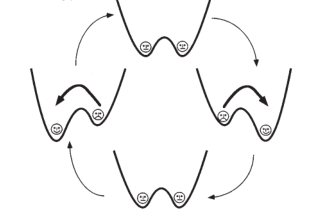
\includegraphics[width=20em]{000.jpg}
\caption{Figure: The first real unmanned vehicle runs on the road.}
\label{fig:lable}
\end{figure}
\par
\section{background}
The first truly autonomous cars �� vehicles that cruise the streets with no one behind the wheel �� have finally arrived.
\par
\section{text}
This week, seven years ago, Google first revealed the prototype of its pilotless technology, shocked the car industry, and then Google invested more than 1 billion in auto driving research.\cite{higham1994bibtex}
\par
Pilotless technology may be one of the most subversive and most hyped new technologies. Unmanned vehicles are the core of a competition between large carmakers and technology companies. But while several groups are testing the technology on the road, with drivers going in the back in case, most still think it will take at least two years to complete automatic driving. Google is still technically ahead, although doubters question whether artificial intelligence technology has been perfect enough to cope with many unforeseeable conditions on the road.
\bibliography{aaa}
\par
\footnote{\centering pilotless automobilen}
\end{document}

